\documentclass{article}

\title{GPU Accelerated Time Series Clustering with Dynamic Time Warping}
\date{\today}
\author{Jeffrey Wong\\MS Student\\Stanford University, Department of Statistics}

\usepackage[pdftex]{graphicx}
\usepackage{amsfonts}
\usepackage[autocite=superscript]{biblatex}

\bibliography{references.bib}

\usepackage{Sweave}
\begin{document}

\maketitle

\newpage

\tableofcontents

\newpage

\section{Introduction}

Time Series Clustering and Classification is a computationally difficult problem
with no clear dominant technique.  In many data mining algorithms a metric for 
dissimilarity between observations is needed; from there, algorithms such as 
k-means clustering and hierarchical agglomerative clustering can be deployed.  
However, for time series data, it is difficult to quantitatively measure how 
similar one time series is to another.  

Since time series data tend to be numeric data, we may consider a time series of 
$n$ time points as a vector in $\mathbb{R}^n$.  This gives the intuition for 
using the Euclidean distance as a dissimilarity metric between two time series.  
However, there are many problems with this: it does not capture the 
overall shapes of the two series, and if one is lagging behind the other
the dissimilarity value will be very large, when it should be small.  

Researchers have recently used an algorithm called Dynamic Time Warping to compare 
numeric time series data.  This algorithm effectively stretches and compresses 
two time series to get the best alignment, then uses a local distance function 
to compute the overall dissimilarity.  Unfortunately, DTW is an $O(n^2)$ algorithm, 
whereas the Euclidean distance runs in $O(n)$.  

In our R package, \textit{TSClust}, we provide functions for using k-means, k-NN, and 
hierarchical agglomerative clustering with Dynamic Time Warping.  This package also
provides fast computations of DTW for many time series through a C implementation
and also a parallel CUDA implementation.  We also generalize R's k-means and dist 
functions to use any distance metric that the user wishes to provide.

\section{Dissimilarity Metrics}

\subsection{Preprocessing and Euclidean Distasnce}

The Euclidean distance, defined as

$$d(x,y) = \sqrt{ \sum_{i=1}^n{ (x_i - y_i)^2 } }$$

is often used to compare numeric vectors in $\mathbb{R}^n$.  However, such a 
metric does not seem suitable for time series data.  For example, suppose we 
have two perfectly sinusoidal patterns generated by $\sin(x)$ and $\sin(x) + 5$:

\begin{Schunk}
\begin{Sinput}
> x = seq(-pi, pi, 0.01)
> y1 = sin(x) + 5
> y2 = sin(x)
> plot(x, y1, col = "red", ylab = "y", main = "sin(x) and sin(x) + 5", 
+     ylim = c(-1, 6))
> points(x, y2, col = "blue")
> legend(min(x) + 1.1, max(y1, y2), c("sin(x) + 5", "sin(x)"), 
+     cex = 0.8, col = c("red", "blue"), pch = 21:22, lty = 1:2)
\end{Sinput}
\end{Schunk}
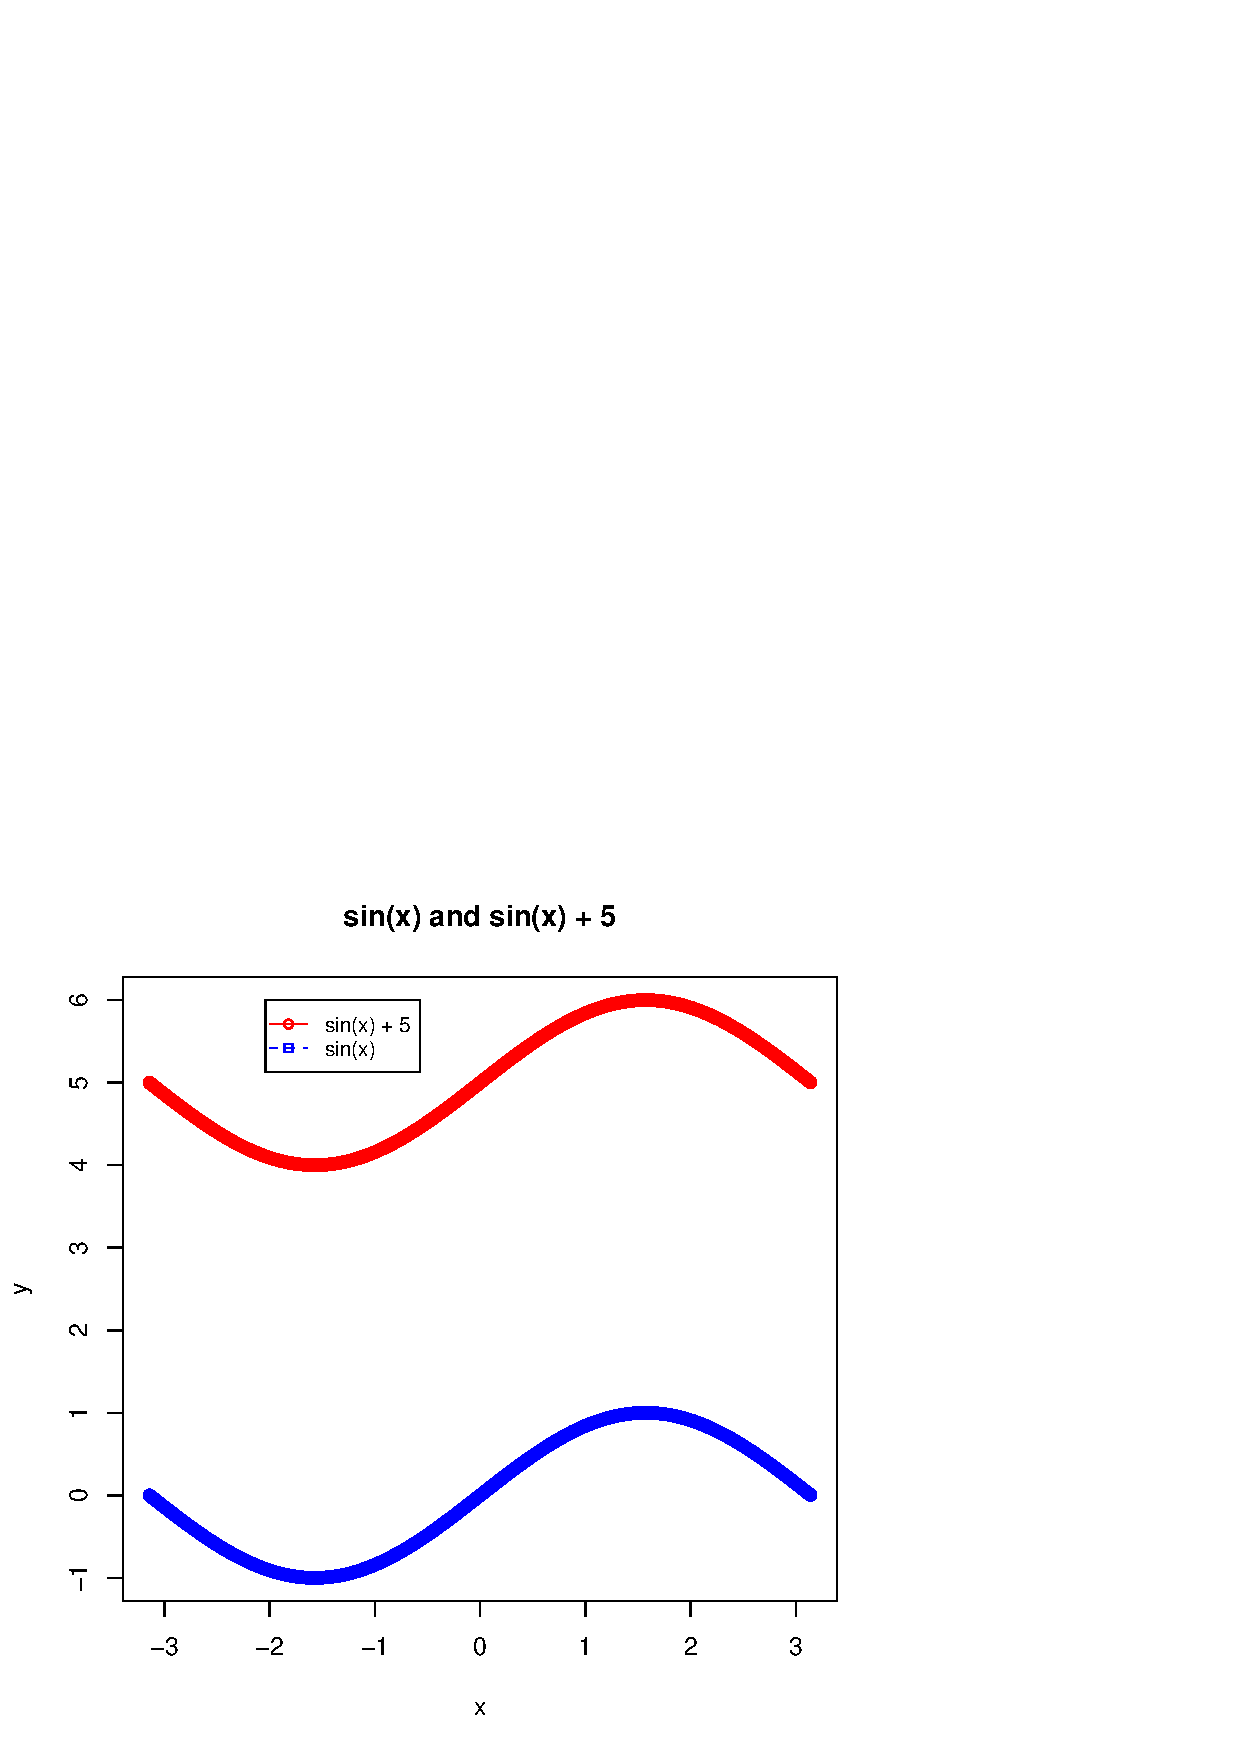
\includegraphics{tsclust-002}

The reported Euclidean distance is 
\begin{Schunk}
\begin{Sinput}
> sqrt(sum((y1 - y2)^2))
\end{Sinput}
\begin{Soutput}
[1] 125.3994
\end{Soutput}
\end{Schunk}

However, we may think that these two time series belong to the same family since
they are perfectly sinusoidal, only differing in a vertical shift.  We may wish 
to define their dissimilarity value as something small.  To eliminate the 
vertical shift, a large contribution to the large Euclidean distance, we can 
preprocess the data and remove the means from the time series.  

Another issue concerns lagged values.  Suppose instead we have two sinusoidal 
patterns generated by $\sin(x)$ and $\cos(x)$.  We know that 
$\cos(x) = \sin(x - \pi/2)$, so we might say that $\sin(x)$ lags behind $\cos(x)$.  

\begin{Schunk}
\begin{Sinput}
> y1 = sin(x)
> y2 = cos(x)
> plot(x, y1, col = "red", ylab = "y", main = "sin(x) and cos(x)")
> points(x, y2, col = "blue")
> legend(min(x) + 1.1, max(y1, y2), c("sin(x)", "cos(x)"), cex = 0.8, 
+     col = c("red", "blue"), pch = 21:22, lty = 1:2)
\end{Sinput}
\end{Schunk}
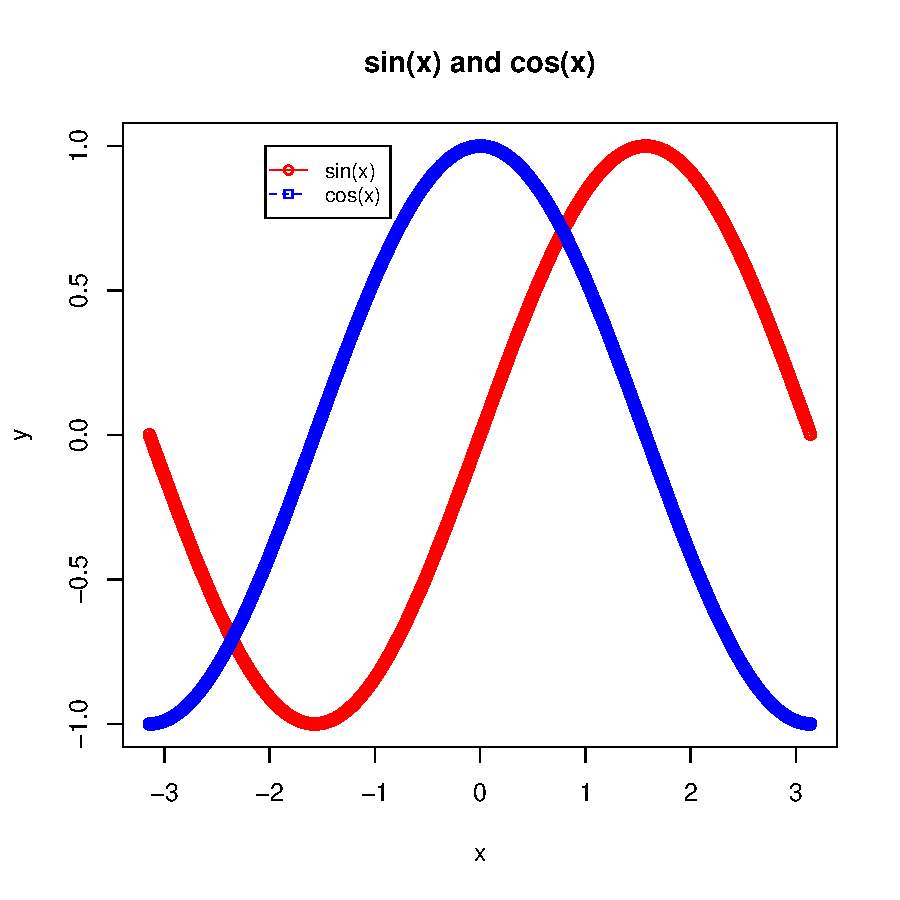
\includegraphics{tsclust-004}

To put this in context, suppose an event $X$ happens at time $t = 0$ and we wish
to see how two different people $y_1$ and $y_2$ respond to it.  $y_1$ and $y_2$
may not immediately respond to event $X$, and furthermore they may not respond 
at the same time.  They may, however, still respond in the same way, i.e. the 
plot of $y_1$ has the same shape and behavior as $y_2$, just horizontally shifted. 
In the case of $\sin(x)$ and $\cos(x)$, both time series have the same amplitude, 
frequency, and local extrema, but $\sin(x)$ is always $\pi/2$ time steps behind 
$\cos(x)$.  Though their Euclidean distance may be large, we may also wish to
define their dissimilarity as something small.

To address this second issue, we introduce a new metric, Dynamic Time Warping.

\subsection{Dynamic Time Warping}

Dynamic Time Warping is an algorithm that stretches and compresses two time 
series along the time axis in order to consider different alignments of the data.
A local distance function is used to compute the dissimilarity between each point
on the series, and the optimal alignment is the alignment that minimizes the sum
of these distances.  

Suppose we have two series, $x$ and $y$, with lengths $n$ and $m$.  Let $d(x,y)$ 
be a local distance function to compare two single points in time.  For simplicity, 
we may consider $d(x,y) = |x - y|$.

DTW may be computed as follows:

\begin{verbatim}
float DTW(x, y, n, m) 
{
  float DTW[n+1][m+1];
  float cost;
  for (i in 1:m)
  {
    DTW[0, i] = INFINITY;
  }
  for (i in 1:n)
  {
    DTW[i, 0] = INFINITY;
  }

  for (i in 1:n)
  {
    for (j in 1:m)
    {
      cost = d(s[i], t[j]);
      DTW[i, j] = cost + min(DTW[i-1, j], DTW[i, j-1], DTW[i-1, j-1]);
    }
  }

  return DTW[n, m];
}
\end{verbatim}

The result is a mapping of the indices from x to the indices of y, and the
distance between each pairwise point according to the local distance function d(x,y).

The R package \textit{dtw} \autocite{DTW} provides computations and visualizations
of the DTW metric.  

\begin{Schunk}
\begin{Sinput}
> y1 = arima.sim(n = 50, list(ar = c(0.8, -0.5), ma = c(-0.23, 
+     0.25)))
> y2 = arima.sim(n = 50, list(ar = c(0.8, -0.5), ma = c(-0.23, 
+     0.25)))
> plot(dtw(y1, y2, k = T), type = "two", off = 5, match.lty = 2, 
+     match.indices = 20)
\end{Sinput}
\end{Schunk}
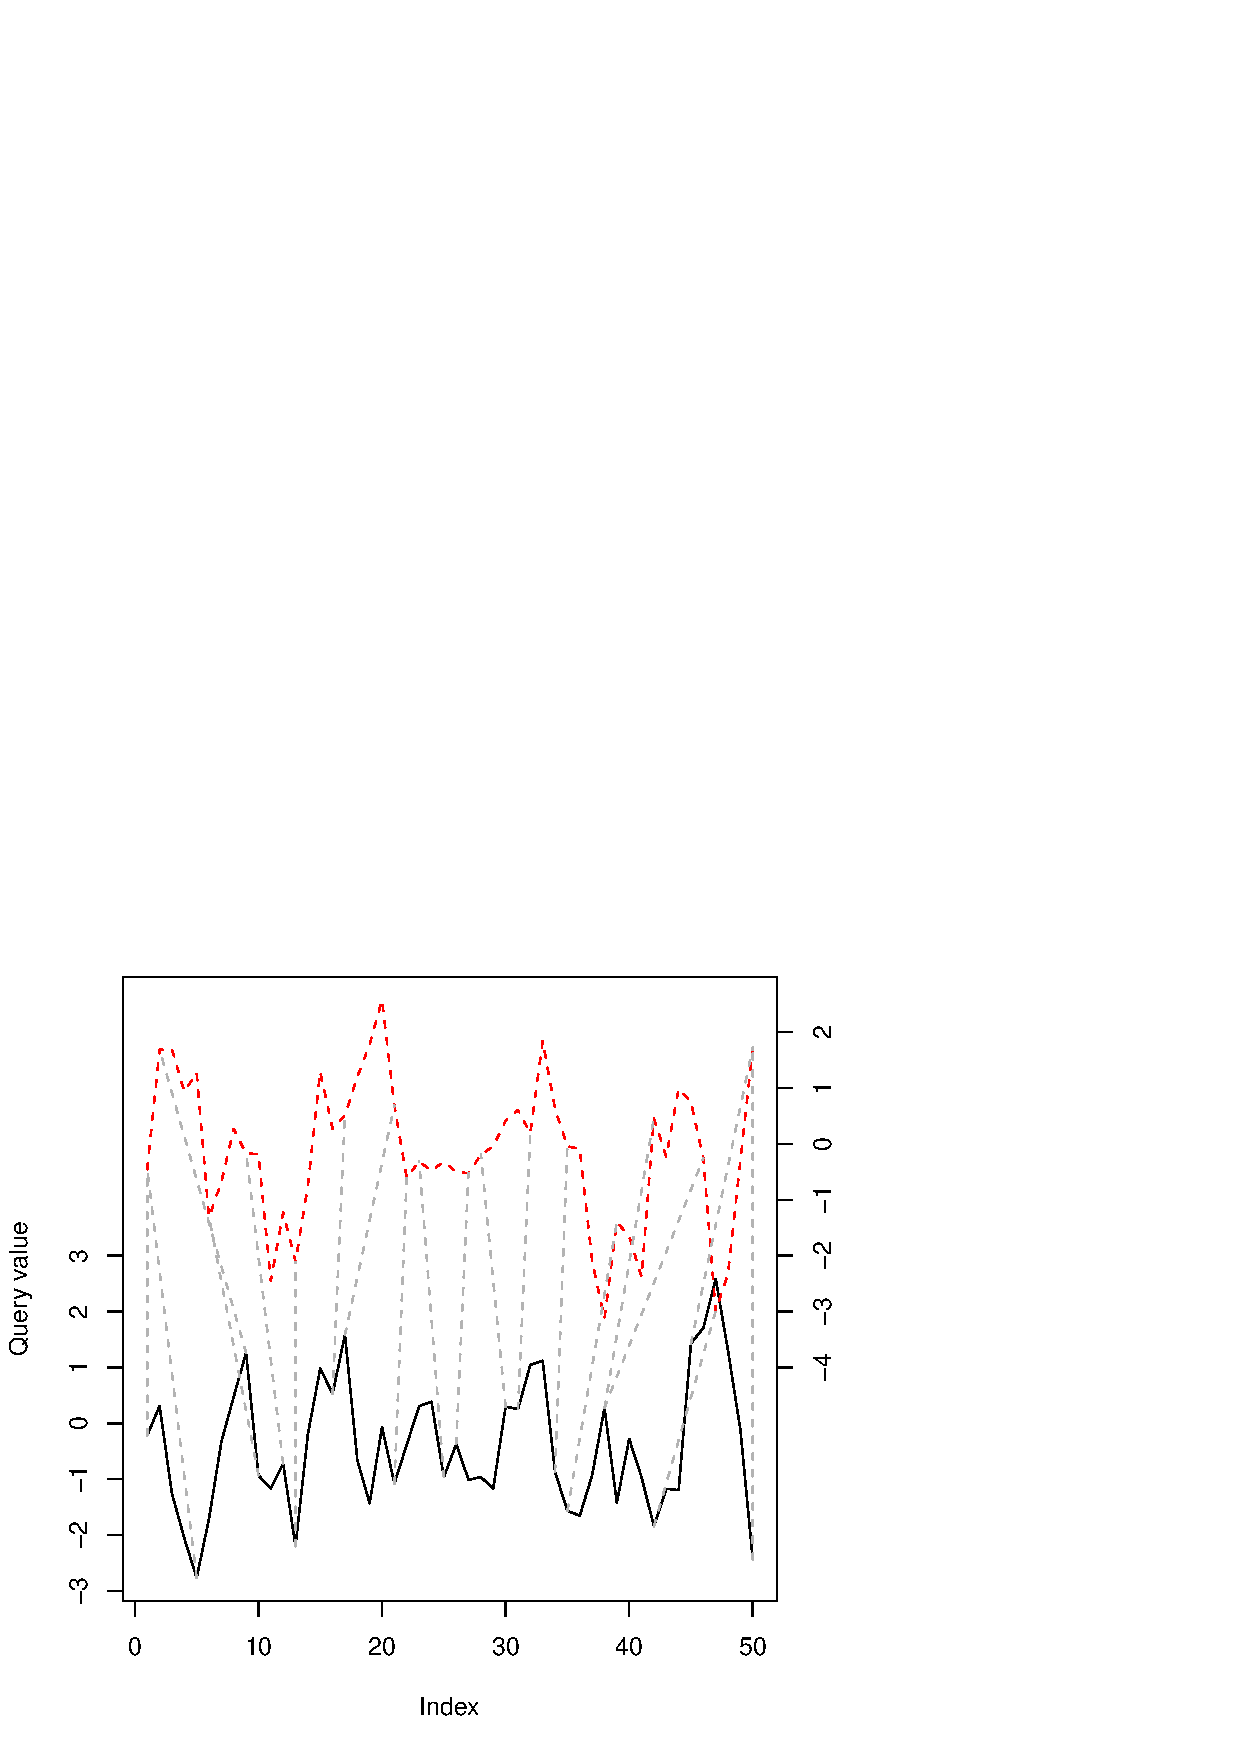
\includegraphics{tsclust-005}

The above figure shows how the indices of the two series are mapped.
The parameters off, match.lty, and match.indices are parameters used for drawing
the two series.

\section{TSClust Algorithms}

\textit{TSClust} provides gpu accelerated time series data mining functions, 
such as clustering using k-means with DTW, classification using k-NN with DTW, 
and hierarchical agglomerative clustering using DTW.  

\begin{itemize}
  \item k-means with DTW
  \item k-NN with DTW
  \item hclust with DTW
\end{itemize}

\subsection{R Implementation}

\subsubsection{tsdist}

In \textit{TSClust}, we generalize the \textbf{dist} function, allowing users
to specificy any distance function in the form

\begin{verbatim}
function(x,y) {
  return distance between x and y
}
\end{verbatim}

The function is then used to compute distances for all possible pairs of 
time series objects in a matrix.  \textbf{tsdist} produces a lower triangular matrix 
of distances, akin to the original \textbf{dist} function.

\subsubsection{tskmeans}

The native R implementation of k-means uses external C code, which limits
the parameters that can be passed in.  tskmeans is a pure R implementation using
the apply family of functions for performance and allows the generalization of the 
k-means algorithm to use any distance function provided.  The user may provide a 
distance function like the one defined above; when computing the distance between 
a time series and a cluster centroid, the provided distance function will be used.

\subsection{CUDA Implementations}

Because DTW has a runtime of $O(n^2)$, it is a highly expensive function to use 
in data mining.  Suppose we have $m$ time series objects we wish to cluster.  
Then a call to k-means has a runtime of $O(mn^2)$, which is furthermore iterated
a number of times until convergence.  Computing the distance matrix is also 
expensive with a runtime of $O(m^2n^2)$.

Both of these algorithms have very clear parallelization strategies.  k-means 
is an EM type algorithm, so we use two CUDA kernels to handle two phases:

\begin{itemize}
  \item Use m CUDA threads to compute the distances between a time series
    object and a cluster centroid
  \item Use n CUDA threads to compute the $i^{th}$ coordinate of the
    cluster centroid in $\mathbb{R}^n$, where $i \in {1 \ldots n}$
\end{itemize}

This CUDA implementation now runs in $O(n^2)$.

Computing the distance matrix can be done by flattening the matrix into a vector.  
For this, we consider the upper right triangular part of the distance matrix, 
with row indices $i$ and columns $j$, such that $j > i$.  The number of pairwise 
distances that need to be calculated is $N = 1 + 2 + \ldots (m-1) = \frac{m}{2} (m-1)$.  
We declare an array of size N to store the pairwise distances, and use N CUDA 
threads to calculate DTW.  Mapping between the two dimensional indices that would
represent the distance matrix and the one dimensional index for the distance
vector can be done with the following:

\textbf{Lemma 1:}  Mapping $i$ and $j$ to an index of a one dimensional array
can be done with the following: the value of the distance between time series $i$ and $j$
should be mapped to the index $x = im - \frac{i+2}{2} (i+1) + j$.

\textbf{Proof:}  Clearly, the mapping function takes the form $x = f(i) + j$.
If we were inspecting a full matrix instead of an upper triangular one, we would have
$f(i) = im$.  We note that in the $i^{th}$ row, $i+1$ cells are left out, so the index is

\begin{eqnarray}
x &=& im - (1 + 2 + \ldots (i+1)) + j\\
  &=& im - \frac{i+2}{2} (i+1) + j
\end{eqnarray}

\textbf{Lemma 2:} Mapping the one dimensional array index to the two dimensional 
distance matrix can be done with the following: the $x^{th}$ CUDA thread 
will compute DTW between time series $i$ and $j$ where 

\begin{eqnarray}
i &=& \frac{-b + \sqrt{b^2 - 4ac}}{2a}\\
j &=& x - im + \frac{i+2}{2}(i+1)
\end{eqnarray}
and
\begin{eqnarray*}
a &=& -1\\
b &=& -1 + 2m\\
c &=& -2x
\end{eqnarray*}

\textbf{Proof:} The first element of the $i^{th}$ row will map to the 
one dimensional index $x = \sum_{k=1}^i (m-k)$.  To find the row that $x$
belongs to, we find the row $i$ where the first element maps to an index $x' > x$.
Then, we step back 1 row and vary $j$ to get the appropriate $x$.  

We wish to find the smallest integer value $i$ such that 

$$\sum_{k=1}^i (m - k) > x$$

Expanding the above equation yields:

$$im - \frac{i+1}{2}i > x$$

Hence $i$ is the floor of the solution to 

$$-i^2 + i(-1 + 2m) - 2x > 0$$

The value of $j$ immediately follows from Lemma 1.

Hence the computation of the distance matrix is drastically improved
from $O(m^2n^2)$ to $O(n^2)$.

\subsection{C Implementation and Memory Issues}

Due to memory limitations on the GPU, some C implementations are still needed. 
DTW is a dynamic programming algorithm, and hence requires a large memory space.
Every calculation of DTW requires allocating memory for $(n+1)$ floats.  
For the above parallel implementation for computing a distance matrix, 
an array of size $\frac{m}{2}(m-1)(n+1)$ is required, not including the array
to store the original data. 

To illustrate, a CUDA enabled GPU with 1 GB VRAM has enough memory to allocate
250 million floats.  The memory space required for a distance matrix is precisely 
$\frac{m}{2}(m-1)(n+1) + mn + \frac{m}{2}(m-1)$.  This is only enough to calculate
a distance matrix for 500 time series of length 2000 each.

\includegraphics{tsclust-006}

The memory requirements for a C implementation are much less, since at any given
time only two time series are being compared, thus reducing the amount of memory
needed.  The memory space required for the same distance matrix is precisely
$(n+1) + mn + \frac{m}{2}(m-1)$.  500 time series objects of length 500,000 
can easily be compared with the expense of 1 GB memory.  

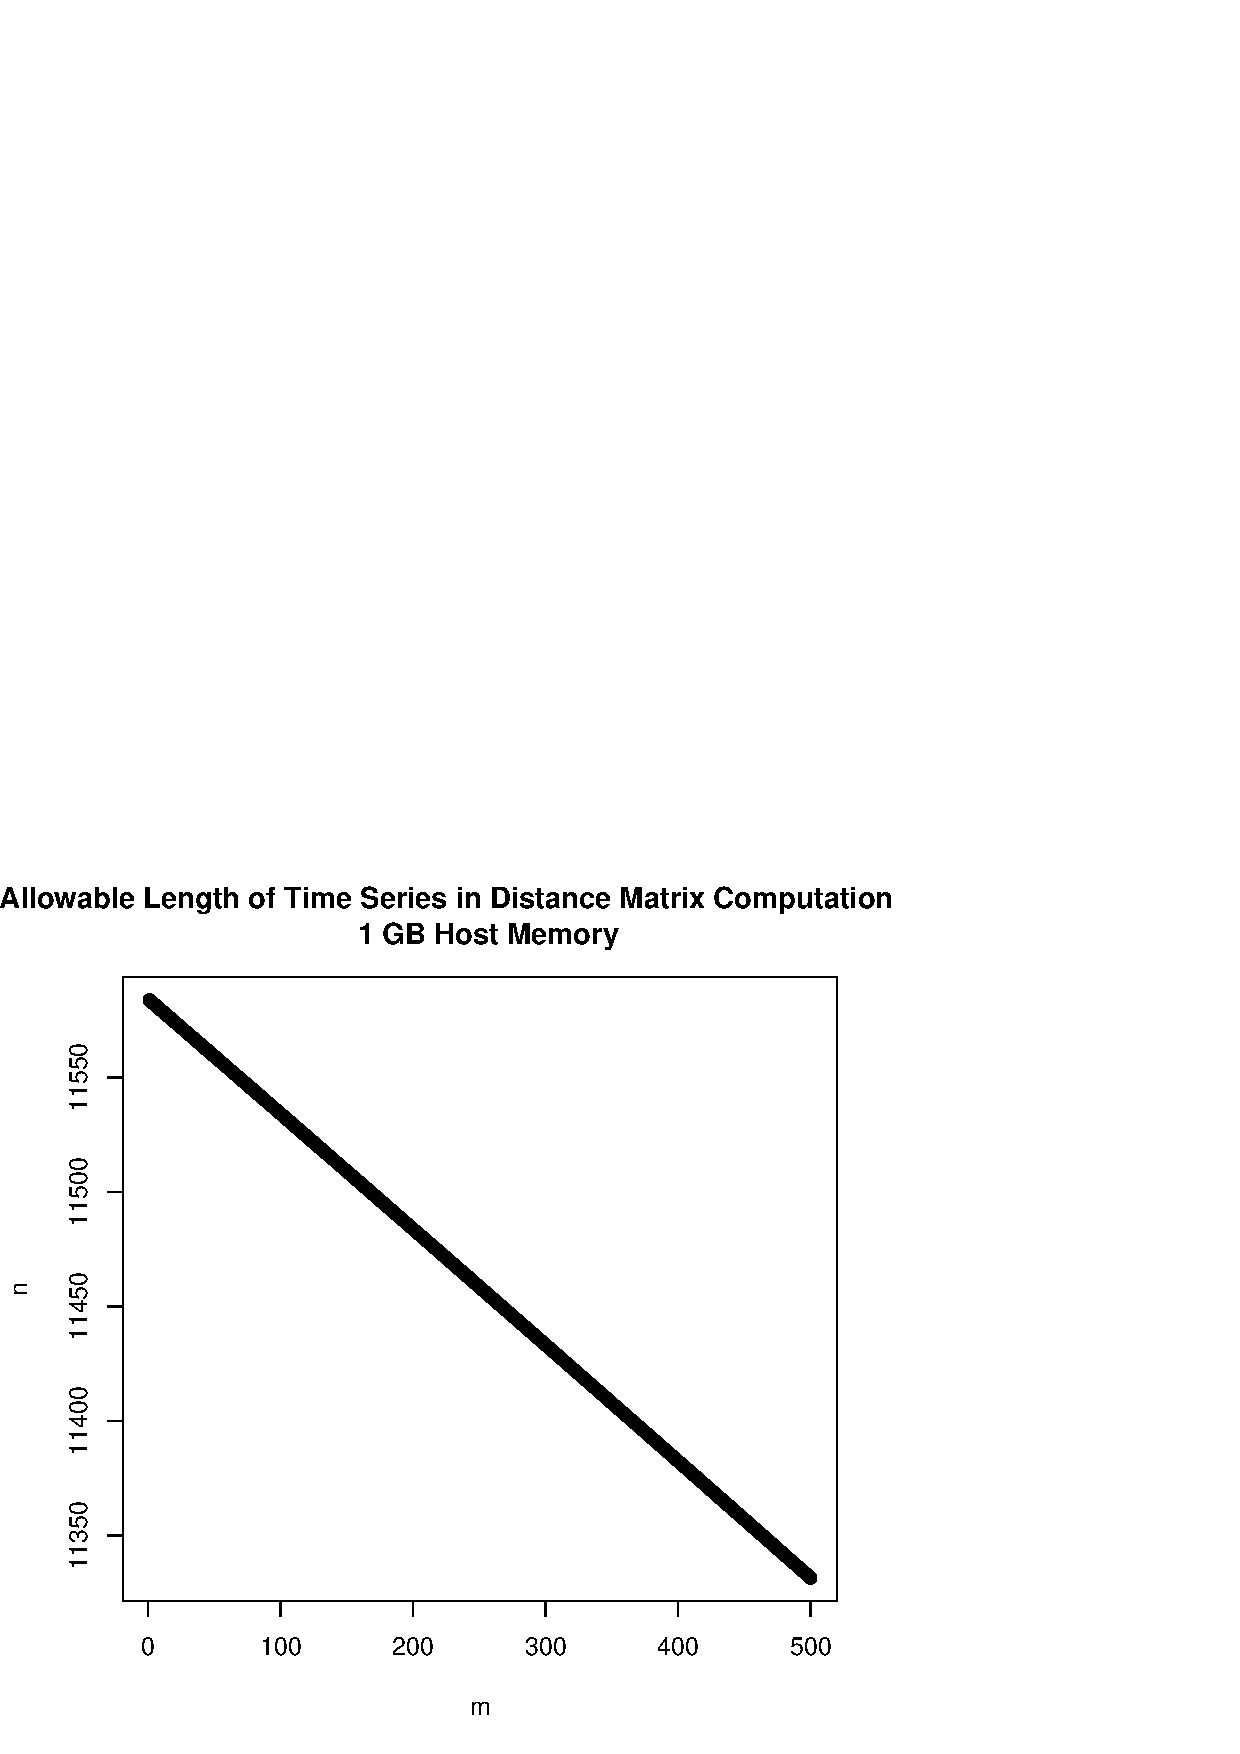
\includegraphics{tsclust-007}

The \textit{dtw} package provides fast C-based methods for computing the
distance matrix, so we can utilize that for computing k-NN and hierarchical
clustering.  A C-based implementation of k-means that uses DTW is still needed,
which is provided in the \textit{src/tsclust.cu} file.

\section{Results}

\subsection{Clustering and Classification}

We will demonstrate the use of tskmeans, tshclust and tsknn here.

First we will generate time series data based off of an ARIMA model
\begin{Schunk}
\begin{Sinput}
> generateTSMatrix = function(clustersizes, tslength, p, q) {
+     k = length(clustersizes)
+     tslist = sapply(1:k, function(i) {
+         clustersize = clustersizes[i]
+         ari = p[[i]]
+         mai = q[[i]]
+         ts.sim = sapply(1:clustersize, function(j) {
+             arima.sim(n = tslength, list(ar = ari, ma = mai))
+         })
+         runif(1, 1, 20) * as.vector(ts.sim)
+     })
+     matrix(unlist(tslist), nrow = tslength, ncol = (length(unlist(tslist))/tslength))
+ }
> set.seed(10)
> x = generateTSMatrix(c(25, 25), 50, list(c(0.8, -0.5), 0.2), 
+     list(c(-0.23, 0.25), 0))
\end{Sinput}
\end{Schunk}

The data clearly contains two clusters.  tskmeans outputs

\begin{Schunk}
\begin{Soutput}
          predicted label
true label  1  2
         1 19  6
         2  7 18
\end{Soutput}
\end{Schunk}

correctly clustering 37 observations.  k-means using Euclidean distance outputs

\begin{Schunk}
\begin{Soutput}
          predicted label
true label  1  2
         1  7 18
         2  0 25
\end{Soutput}
\end{Schunk}

correctly clustering only 32 of the 50 time series.

From tshclust with DTW, we can generate a tree which clearly shows 2 clusters
with nearly equal sizes

\begin{Schunk}
\begin{Sinput}
> set.seed(10)
> x = generateTSMatrix(c(25, 25), 50, list(c(0.8, -0.5), 0.2), 
+     list(c(-0.23, 0.25), 0))
> x.dist = tsdist(x)
> x.hclust = hclust(x.dist)
> plot(x.hclust)
\end{Sinput}
\end{Schunk}
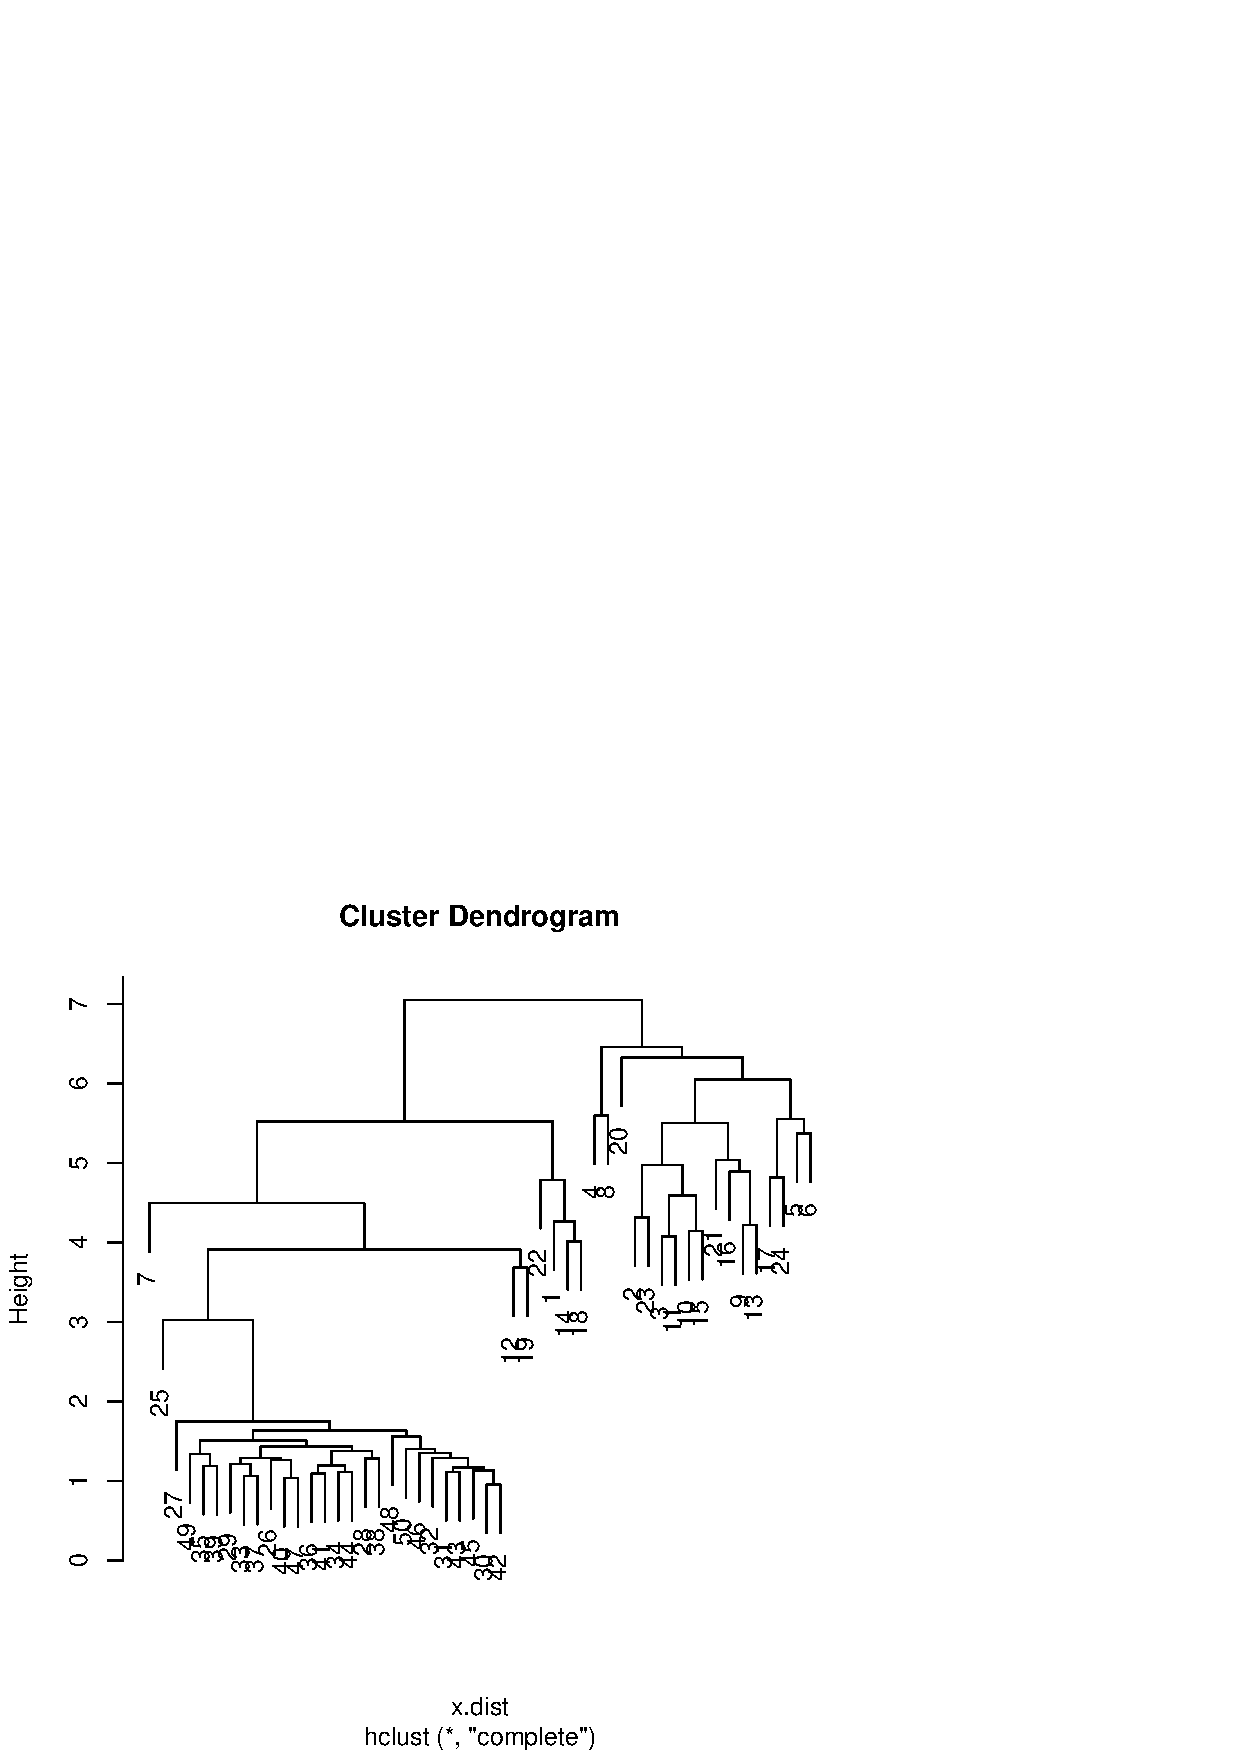
\includegraphics{tsclust-011}

Only observations 7 and 25 are misclassified.  

With the Euclidean distance, one cluster is significantly smaller than the other

\begin{Schunk}
\begin{Sinput}
> x.dist = dist(t(x))
> x.hclust = hclust(x.dist)
> plot(x.hclust)
\end{Sinput}
\end{Schunk}
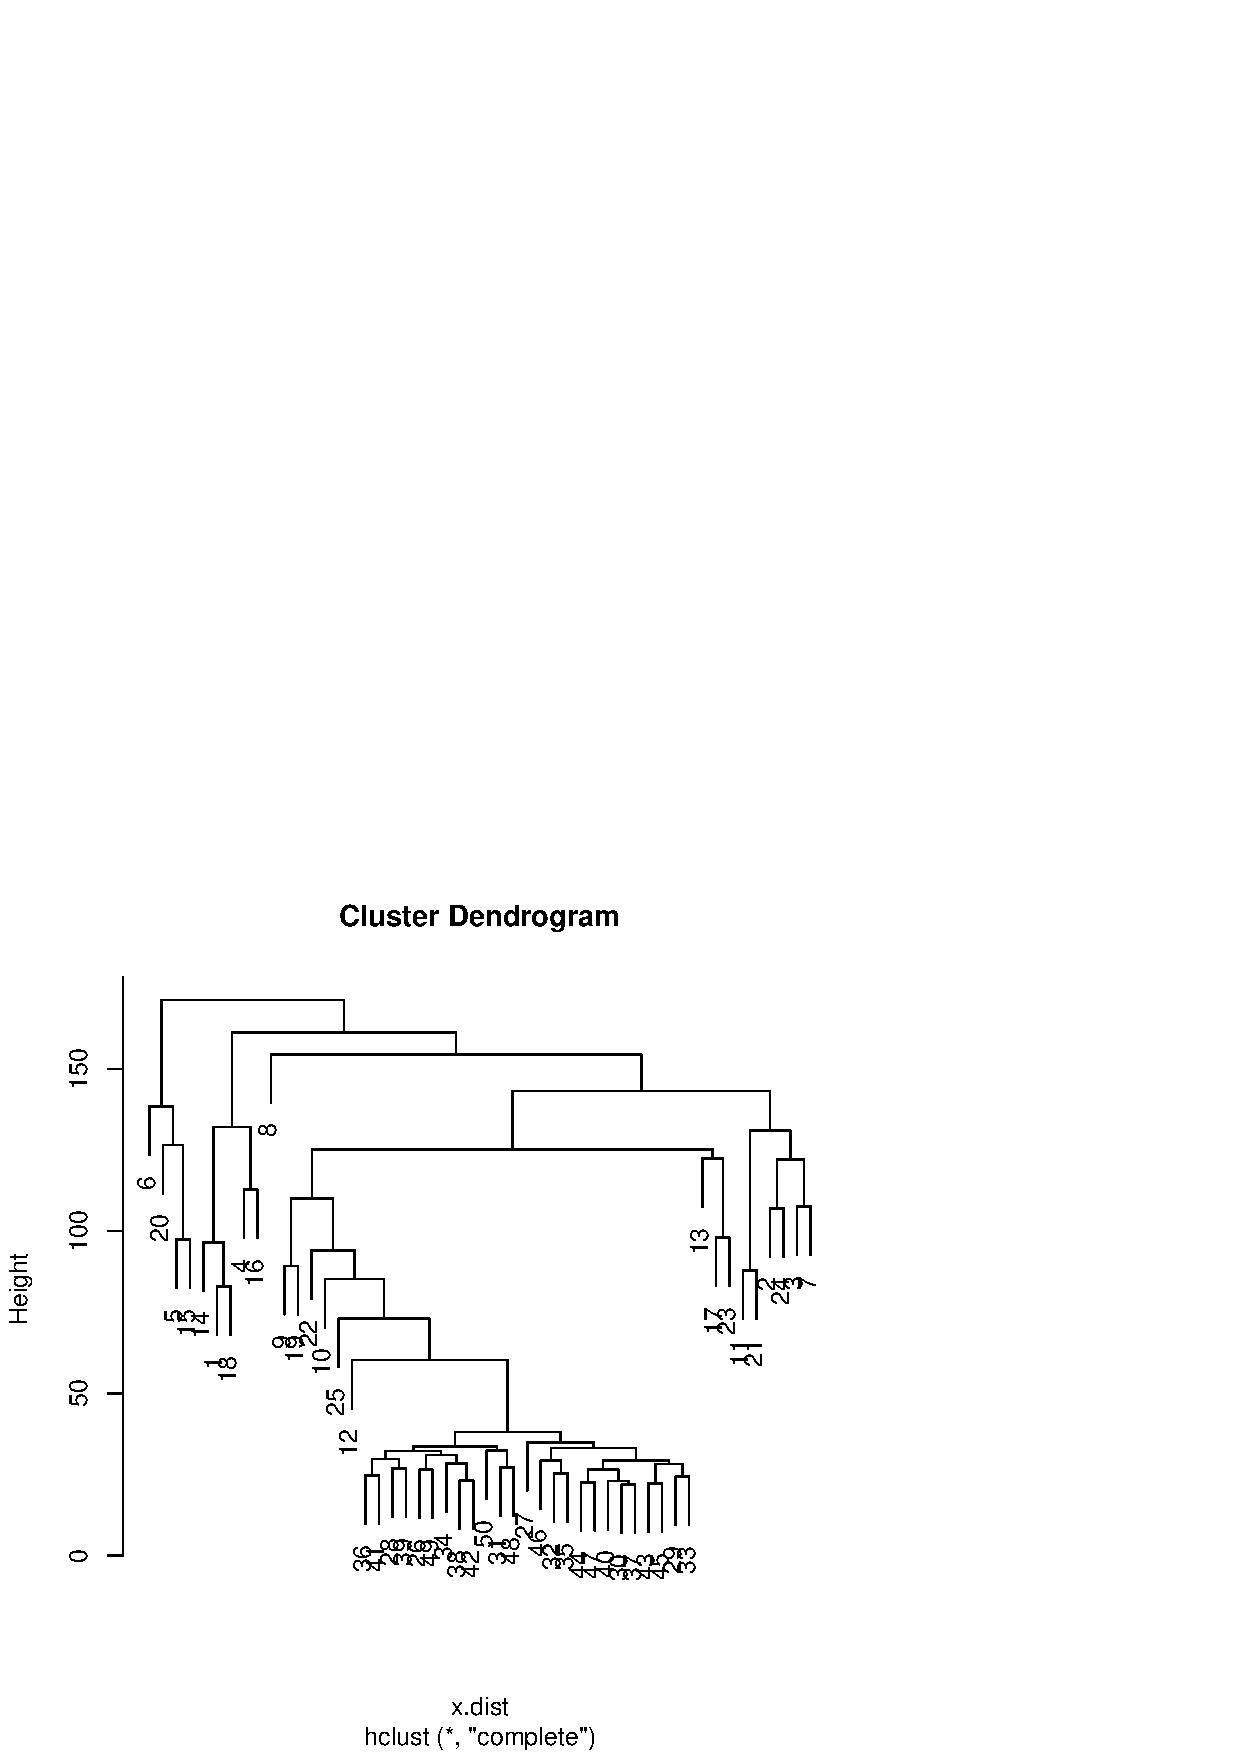
\includegraphics{tsclust-012}

\subsection{Runtime}

We can stress the kmeans algorithm by using 500 time series objects of length 1000 each.
The runtimes for the R implementation, CUDA implementation, and C implementation are

\begin{Schunk}
\begin{Sinput}
> system.time(tskmeans(x, k = 2, method = "R"))
\end{Sinput}
\begin{Soutput}
    user   system  elapsed 
4807.110   81.320 4888.417 
\end{Soutput}
\begin{Sinput}
> system.time(tskmeans(x, k = 2, method = "CUDA"))
\end{Sinput}
\begin{Soutput}
   user  system elapsed 
126.640   0.850 127.557 
\end{Soutput}
\begin{Sinput}
> system.time(tskmeans(x, k = 2, method = "C"))
\end{Sinput}
\begin{Soutput}
   user  system elapsed 
 241.49    0.01  241.50 
\end{Soutput}
\end{Schunk}

\section{Conclusion}

In summary, \textit{TSClust} provides functions for time series clustering 
and classification using Dynamic Time Warping.  Through repeated trials, we
have found that k-means clustering using DTW has an average successful clustering 
rate of $78\%$; k-means clustering using the Euclidean distance had an average 
successful clustering rate of $55\%$.  tshclust had a $10\%$ misclassification
rate and k-NN with DTW had a misclassification rate of only $12\%$.

\section{Future Work}

\begin{itemize}
  \item Cluster level implementations of TSClust to handle very large datasets
\end{itemize}

\printbibliography

\end{document}
